\section{Contract based perception algorithms}
\label{delayErrorCurve}

In Section \ref{sec:codesign}, we postulated the existence of an Estimation Error vs Computation Delay curve $\Delta$. % (the `error-delay curve').
This curve is used at every time step by the controller to determine the operating point $(\delta,\epsilon)$ for the next time step.
In this section we demonstrate in detail how such a curve may be obtained for particular applications and how points along the curve are realized at runtime by the contract based perception algorithms.

\subsection{Profiling And Creating an Anytime Contract Based Perception-and-Estimation Algorithm}
\begin{figure}[htbp]
	\centering
	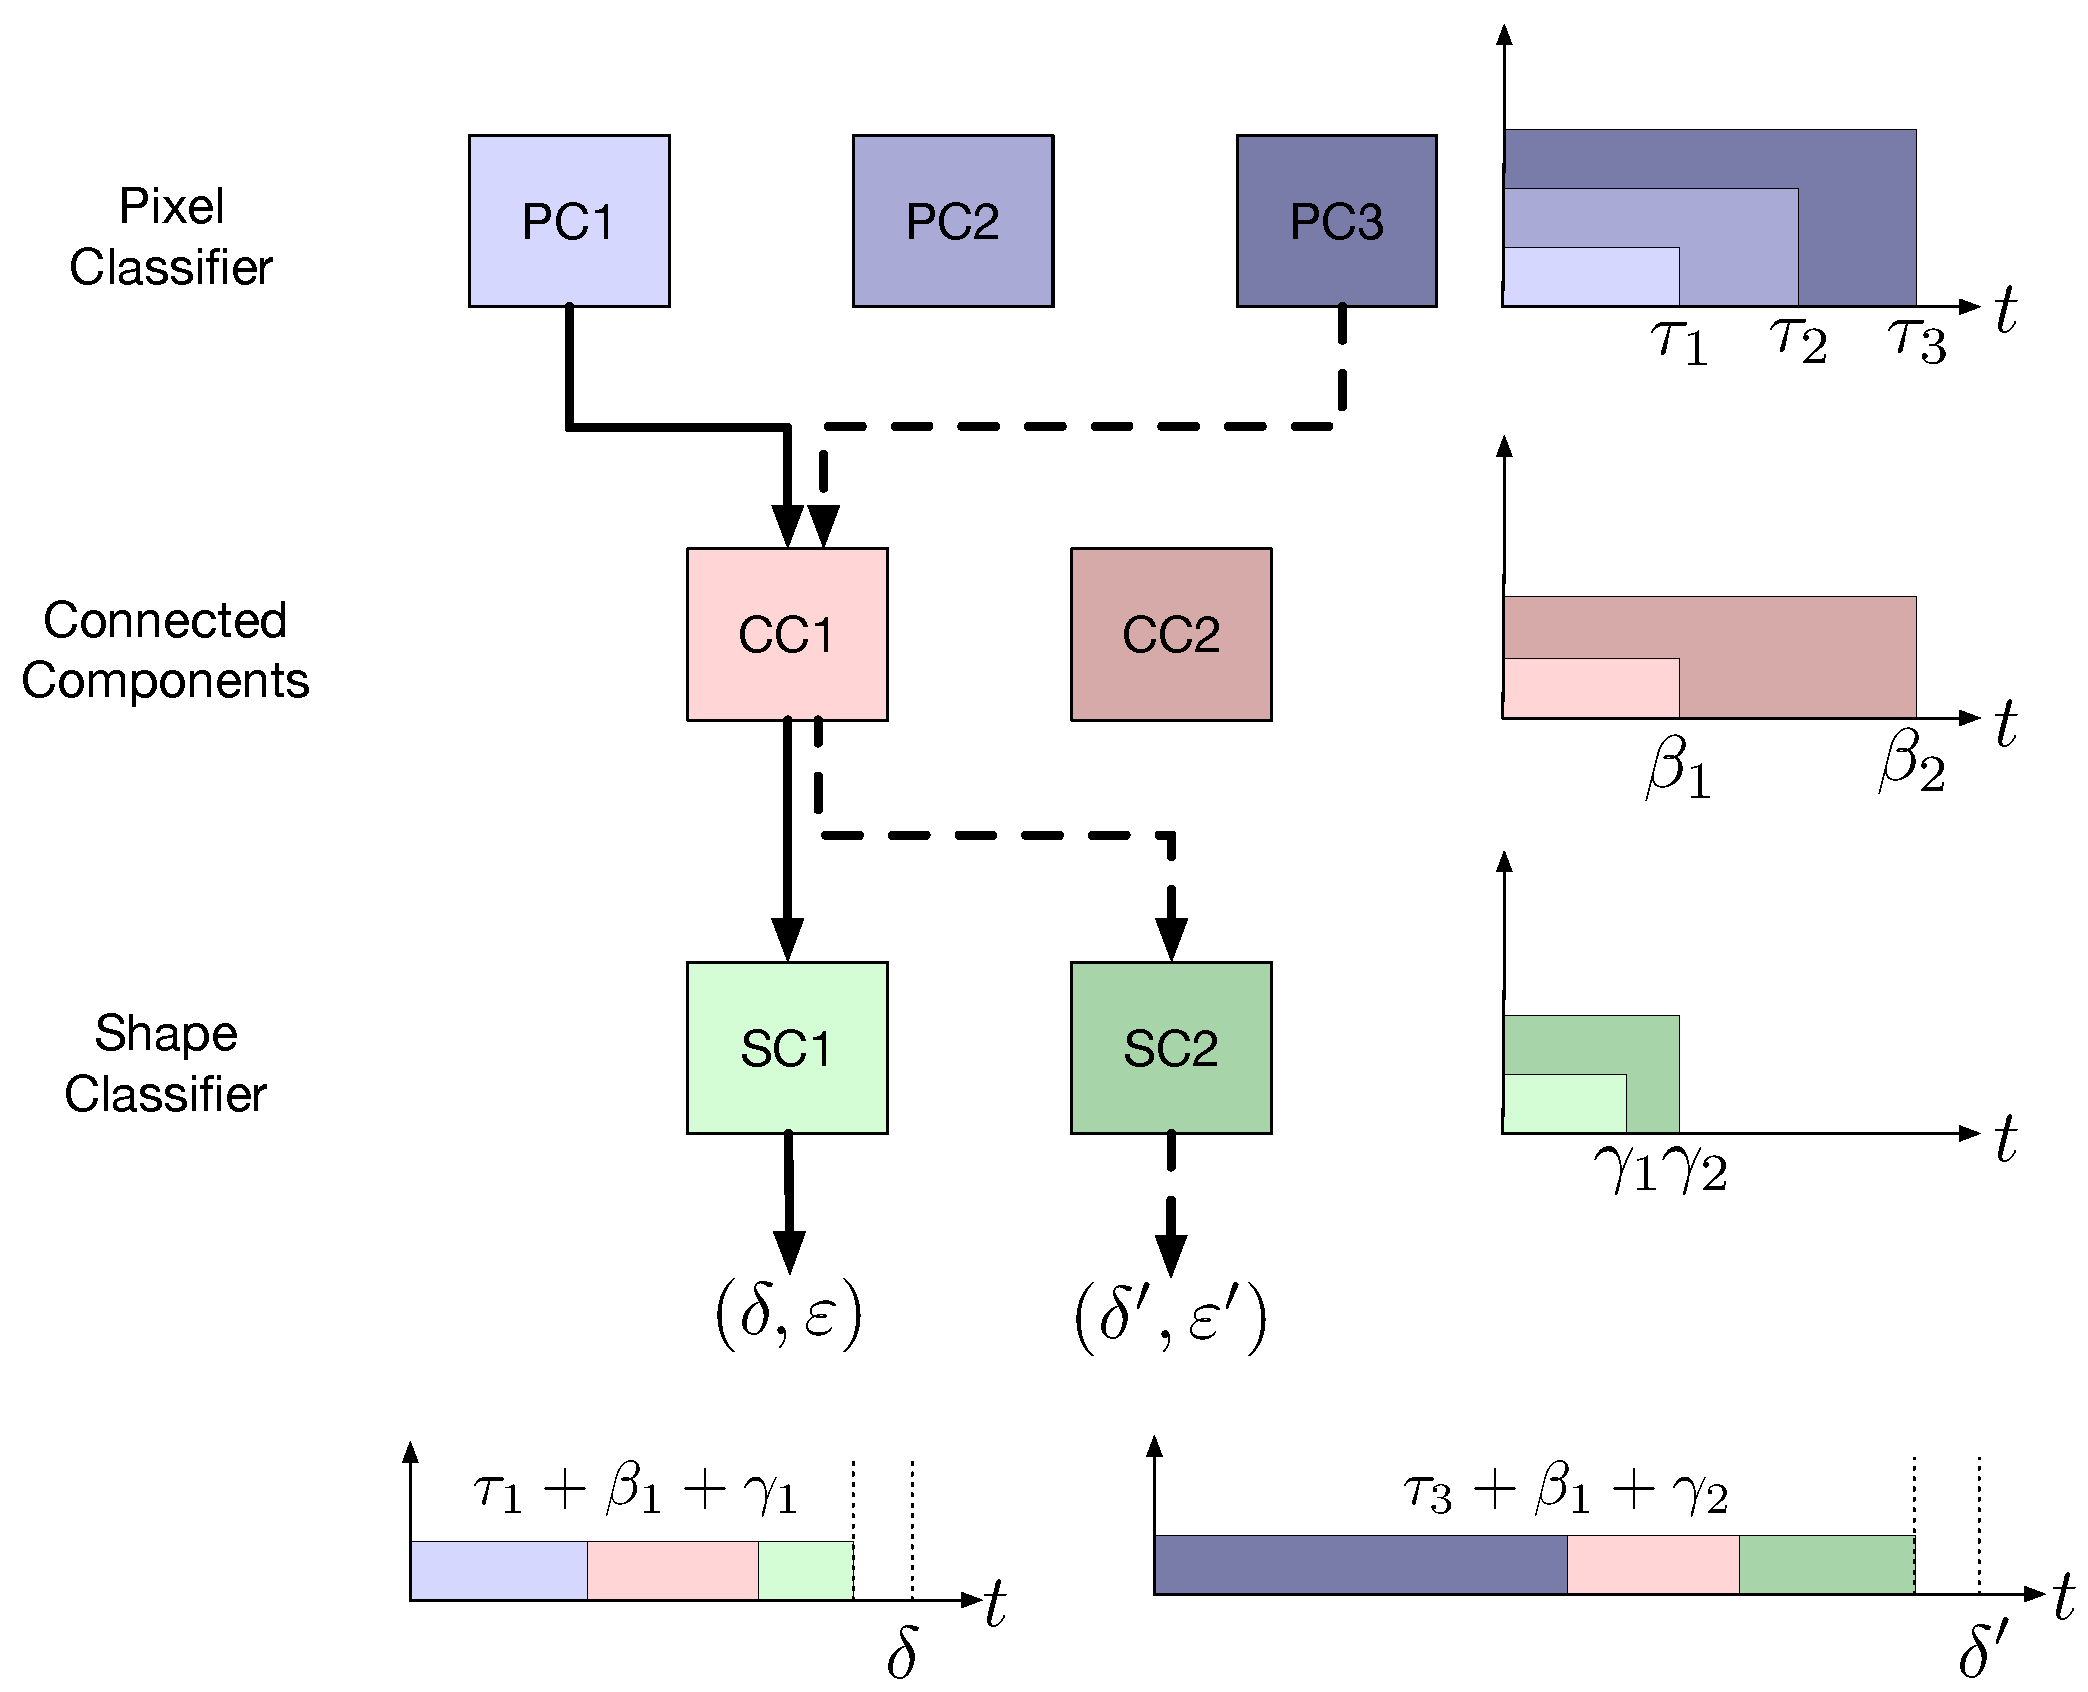
\includegraphics[width=0.49\textwidth]{figures/omnigraffle_figures/real_time_figure}
	\caption{Illustration of the various components used to compose the contract based perception algorithm and their representation as real-time tasks. For a given $\de$ contract, knob settings are chosen at run-time resulting a schedule to execute these sequential components, or tasks to respect the contract.}
	\label{fig:RT_bs}
\end{figure}
The first step towards profiling a contract-based estimator is to identify the individual components (or algorithms) of the perception tool chain. 
The second step is to identify parameters of each component, such that modifying the values of these parameters leads to a change in the execution time and accuracy of the component's output.
This may be as simple as changing the number of iterations in a loop \cite{loop-perf} or finding alternate implementations with different resultant execution times $\sDelay$ and estimation error $\sAccu$.
We call these parameters \emph{knobs} of the component.
The tool chain 
We implement this procedure on a Computer Vision (CV)-based object recognition tool chain. 
An overview of the tool chain is shown in Fig. \ref{fig:RT_bs}.

The CV tool chain takes in a video stream and tracks an Object Of Interest (OOI) across the frames. 
The first stage of the chain is a pixel classifier that assigns to each pixel of the image (after potential pre-processing) the probability of its being a pixel of interest, i.e., of belonging to an OOI or being a part of the background. 
A binary image is then obtained which assigns the value 1 to pixels of interest, and 0 to all others. 
Next, filtering and a Connected Components (CC) algorithm is run on the binary image to get rid of noise in the classification process and segment its 1-valued pixels into disconnected objects. 
A shape classifier is then run on each object to determine whether it is an object of interest or not.
%A knob here in the pixel classification stage is to realize different computation time and performance profiles, is the complexity of the probabilistic model used to detect whether a pixel belongs to the object of interest. The knob in this case is whether we choose a Gaussian Mixture Model (GMM) with fewer components, which would be faster but less accurate, versus a GMM with more components which will take more computation time but provide better classification performance. Knobs where we over fit the training data are removed by cross-validation stage as is standard.

In our implementation, the pixel classifier is a Gaussian Mixture Model (GMM) classifier, whose knob is the number of components in the GMM. 
Fewer Gaussians in the GMM yield a faster but less accurate classifier while more Gaussians will result in a higher execution time but provide better classification performance. 
Knob values that cause data overfit are discarded by a cross-validation stage as is standard.

The filtering and Connected Components algorithm are lumped into one stage and have a two-valued knob to choose between a 4-connected and 8-connected component implementation. 
The shape classifier is also a GMM, but the knob for it is the number of shape features (like eccentricity and lengths of major and minor axes).
%, resulting in Gaussians in different dimensions being fit, and hence resulting in different computation time and classification accuracy.
% The number of Gaussian components for the shape classifier is fixed since we know in advance the number of objects in the training and test sets.
In our experiments the number of knob settings for the entire chain is $K$ = (\#Gaussians for pixel classifier, \#neighbors for CC, \#features for shape classifier), and has a total of $3 \times 2 \times 2 = 12$ values.

Note that for any given component in the chain, the relation between knob value and quality of output is not necessarily monotonic. The pixel and shape classifiers are machine learning algorithms that need to be trained on a training set before being used and like all machine learning algorithms, their output quality for a given knob setting will depend on the actual data set.
The same is a fortiori true of the quality of the output of the entire chain. This is also reflected in Fig.~\ref{fig:eps_delta_toy} which shows the mean perception error\footnote{Error is the distance between the true centroid and the estimated centroid of the OOI} and the $90^{th}$ percentile execution time for the different knob settings. 

The final step is to profile all the possible combinations of knobs by running the tool chain on a test data set.
This profiling gives us: a) the output quality (or accuracy) of the perception-and-estimation tool chain under consideration, and b) information about execution times for the stages of the perception tool chain under different knob settings. 
This information gathered offline is useful for making decisions at run-time. 
Fig. \ref{fig:eps_delta_toy} shows the profiled performance of the CV tool chain.

%Note, since intermediate qualities are not easily measurable or assignable for some of the blocks of the tool chain (e.g. Connected Components) and for many other algorithms in general, we assign quality (or accuracy) distributions to the realizations of the complete tool chain by composing together different knob settings. Note, this profiling stage is done at offline at design time and provides us information that we use at runtime.

\subsection{Run-time execution of the contract based perception algorithm}

After the contract based perception algorithm has been composed and the execution time distributions of its individual components and the quality distributions from composing together various knob settings have been profiled, we can make run-time decisions for knob settings in order to realize a given $\de$ contract. 

%The decision of selecting which knob setting to use for a particular stage for a given criteria can now be posed as an optimization problem for edge selection in the decision tree. For example, consider the case where we want to minimize the perception error while meeting a time deadline with a given high probability, the problem can be written as a constrained minimum cost path selection problem where timing information of the edges and quality information about paths can easily be encoded. This problem can be re-solved after each stage is executed with a recalculated time remaining and smaller decision tree structure for subsequent remaining stages. This allows the algorithm the flexibility to re-optimize its execution path (or knob settings) after obtaining updated information on time consumed in the past stages. For problems that do not have an excessively large number of knobs, such an optimization can be solved very quickly.

This is the equivalent of selecting different versions of tasks (knobs for stages) and scheduling them in sequential order to best perform the object recognition task while maximizing utilization (or estimation accuracy) and meeting the given time contract or deadline. Fig. \ref{fig:RT_bs} shows the different task versions for each knob in the different stages and the resulting schedule based on the knob settings for the stages. The offline profiling allows us to set the knobs such that we can achieve a feasible schedule for the given deadline, $\delta$ while maximizing the utility, or the expected accuracy of the perception algorithm. 

\begin{figure}[t]
	\centering
	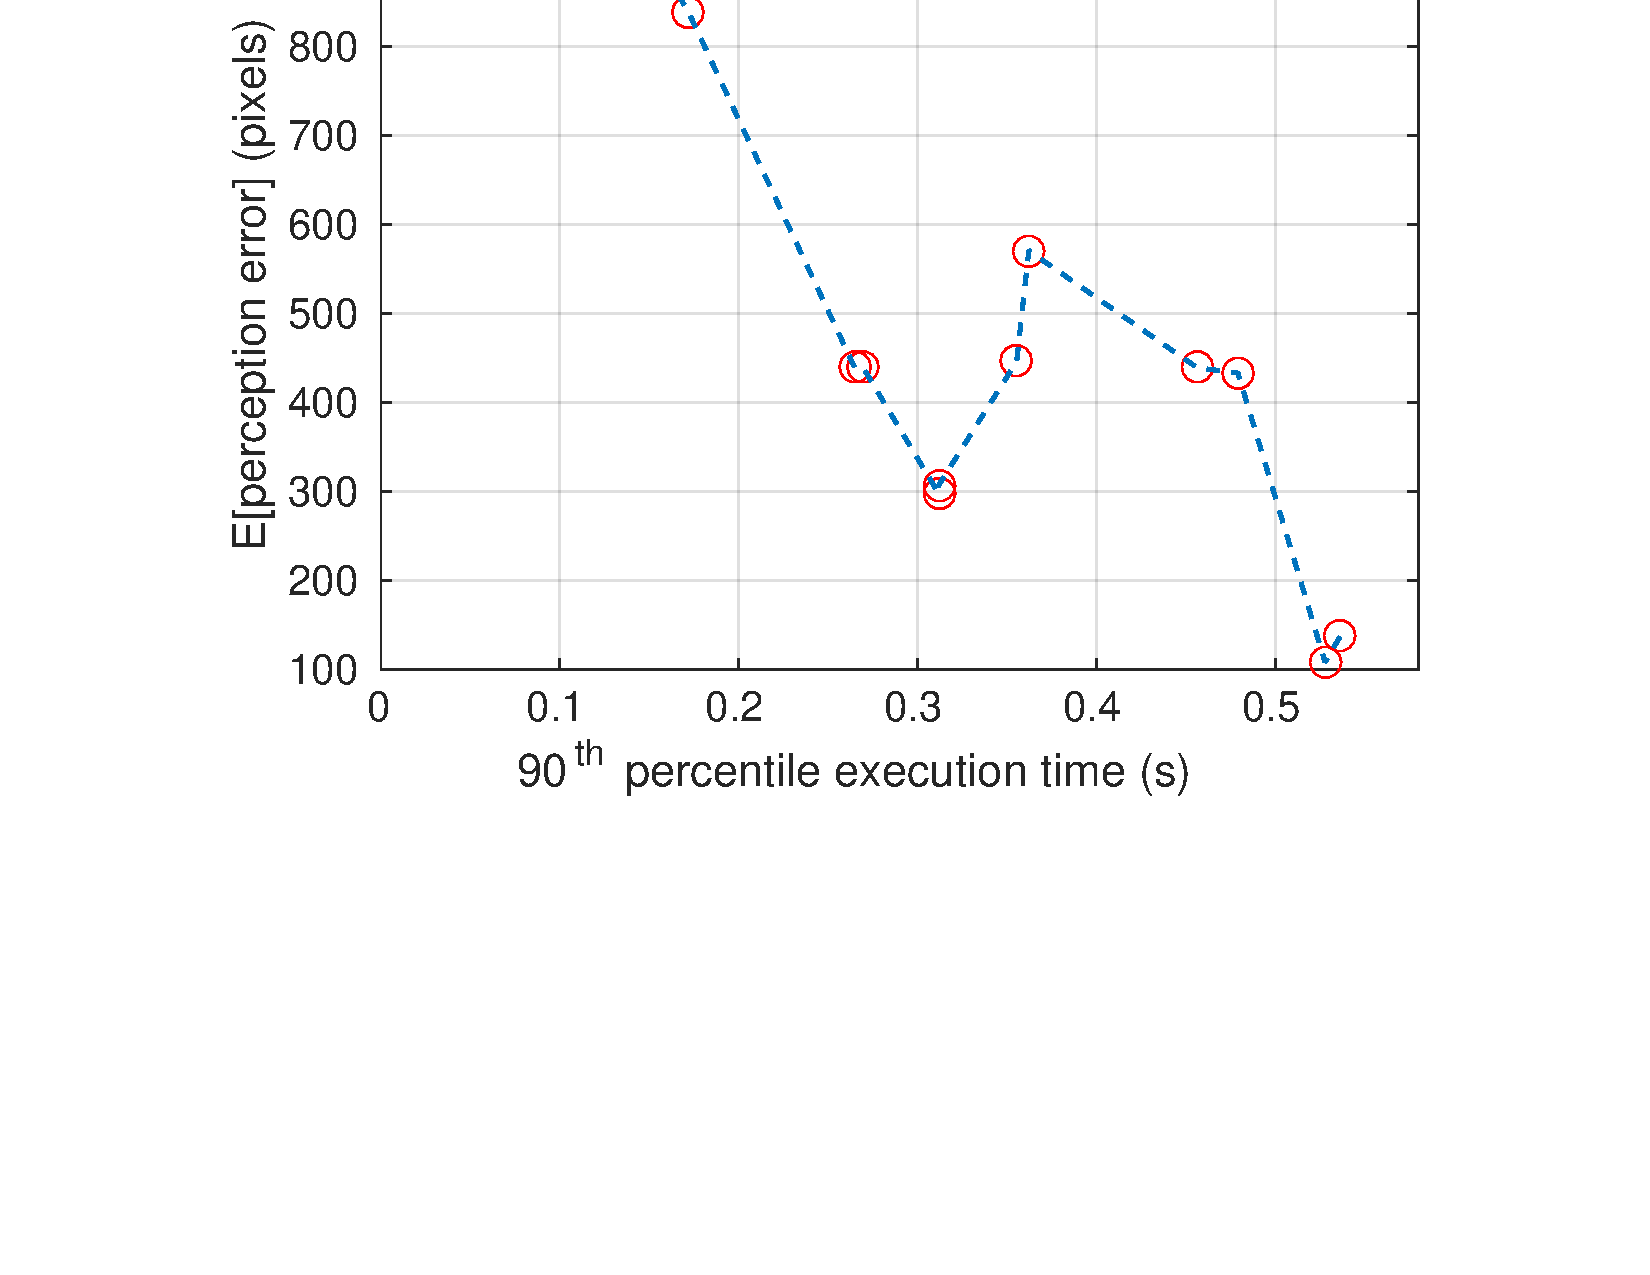
\includegraphics[trim = 0 30mm 0 30mm, width=0.49\textwidth]{figures/chainErrorDelay}
	\caption{Profiled delay-error curve for the object detection tool chain run at different parameter settings.}
	\label{fig:eps_delta_toy}
\end{figure}




%Specifically, we consider two different visual perception tool chains, where each tool of the chain has a knob that tunes its performance.%
%These knobs can be used to profile the tool chain and obtain its error-delay curve on particular platforms.
%Because power consumption is correlated to computation time, the error-delay curve can also be viewed as an error-power curve.
%The power consumption of the estimator task can be included in the control cost function using the $\alpha$ term of Eq.??.
%Thus, the controller can save power by selecting operating modes $(\delta,\epsilon)$ that achieve the control objectives at a lower energy cost.



% subsection
\subsection{Visual Odometry}

Another algorithm we consider is the Semi-Direct Monocular Visual Odometry (SVO)\cite{forster2014svo} which is used for estimating the position and orientation of the hexrotor using an onboard downward facing camera (see section \ref{sec:experiments}).
The visual odometry algorithm detects corners in an image and tracks them across video frames to perform self-localization of a moving robot.
These estimates are used in the closed loop control system that flies the hexrotor, hence it is important for the visual odometry to run at or faster than frame rate in order to provide a timely state estimate to the control algorithm
The number $\#C$ and quality of corners detected in a frame directly affects the runtime of the corner detector and the resulting quality of the state estimate. Generally speaking, detecting more corners requires a longer runtime, and results in better self-localization as long as we are analysing a feature rich scene, i.e., \emph{assuming acceptable quality of the detected corners}. Thus the number $\#C$ of corners is a knob which can be varied to obtain an error-delay curve for self-localization with the visual odometry algorithm.
If the scene is not rich enough in features, and a sizeable fraction of the $\#C$ corners are of poor quality (i.e., unstable or hard to track across frames), then we can expect the self-localization error to actually increase as the poor quality of the unstable corners detected adds noise to the visual odometry estimates.

Fig.~\ref{fig:svo_err_delay} shows the error-delay curve of self-localization error using the SVO.
The curve was obtained on an Odroid-U3 [??], which is the same processor as the one used on the hexrotor for on-board computation.
For each value of the knob $\#C$ (i.e., each requested number of corners), we ran the visual odometry algorithm on a video sequence recorded by the downward facing camera on the hexrotor while flying certain pre-set patterns.
Ground truth for computing the self-localization error was obtained using a Vicon motion capture system which provides position estimates with better than millimeter level precision.
As we repeat each flight several times, this results in a distribution of $(\delta,\epsilon)$ values for each value of $\#C$.
We retained the $90^{th}$ percentile values for $\delta$ and $\epsilon$, since these are used as worst-case estimates by the controller of Section \ref{controlProblem}.
It can be seen that a larger number of requested corners produces a smaller estimation error and longer runtime.
Starting at 250 corners, the error increases, however.
We hypothesize this is due to the decreasing quality of the corners being returned by the corner detection algorithm.
\begin{figure}[t]
\centering
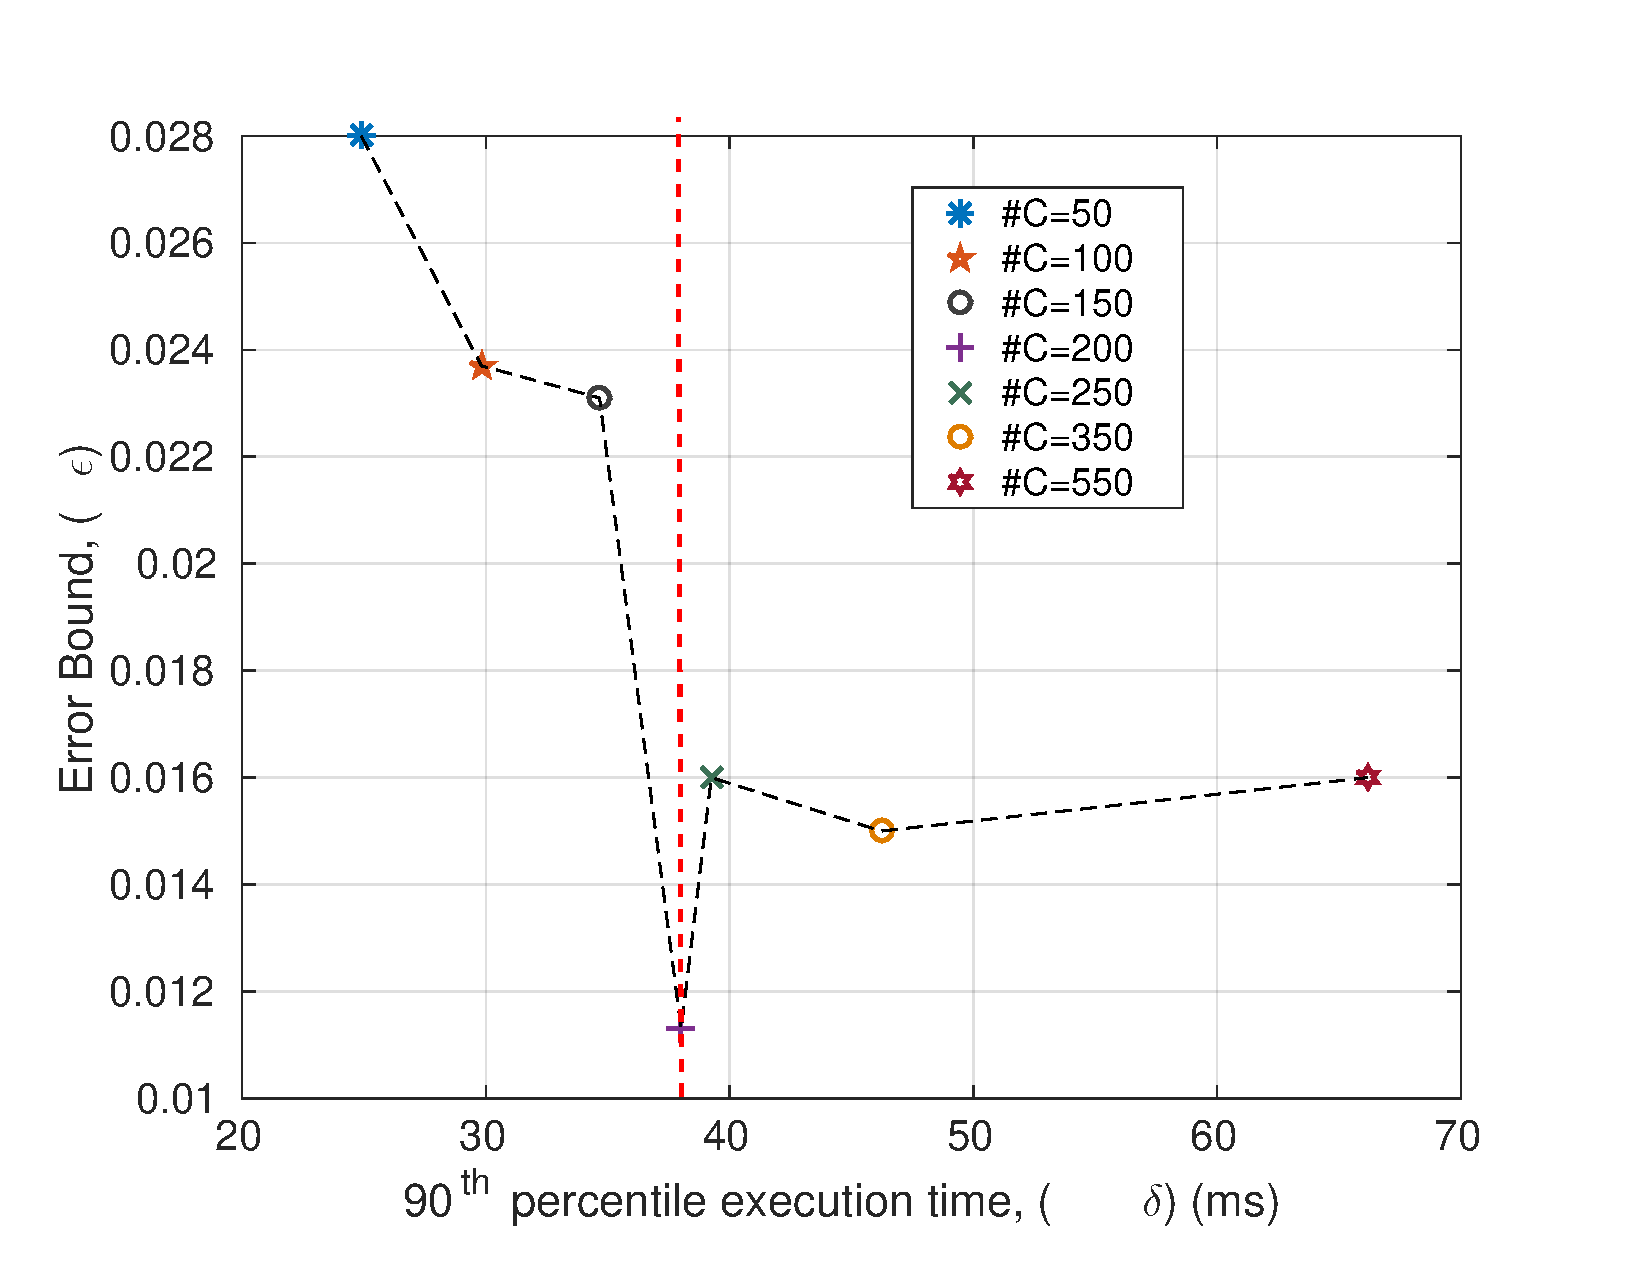
\includegraphics[width=0.9\columnwidth]{figures/errVsTime}
\caption{Error-delay curve for the SVO algorithm running on the Odroid-U3 - ?? Label where we stop choosing delays}
\label{fig:svo_error_delay}
\end{figure}

Fig.~\ref{fig:svoErrVsPower} shows the power consumption vs estimation error, which correlates well with Fig.~\ref{fig:svo_error_delay}.
\begin{figure}[t]
	\centering
	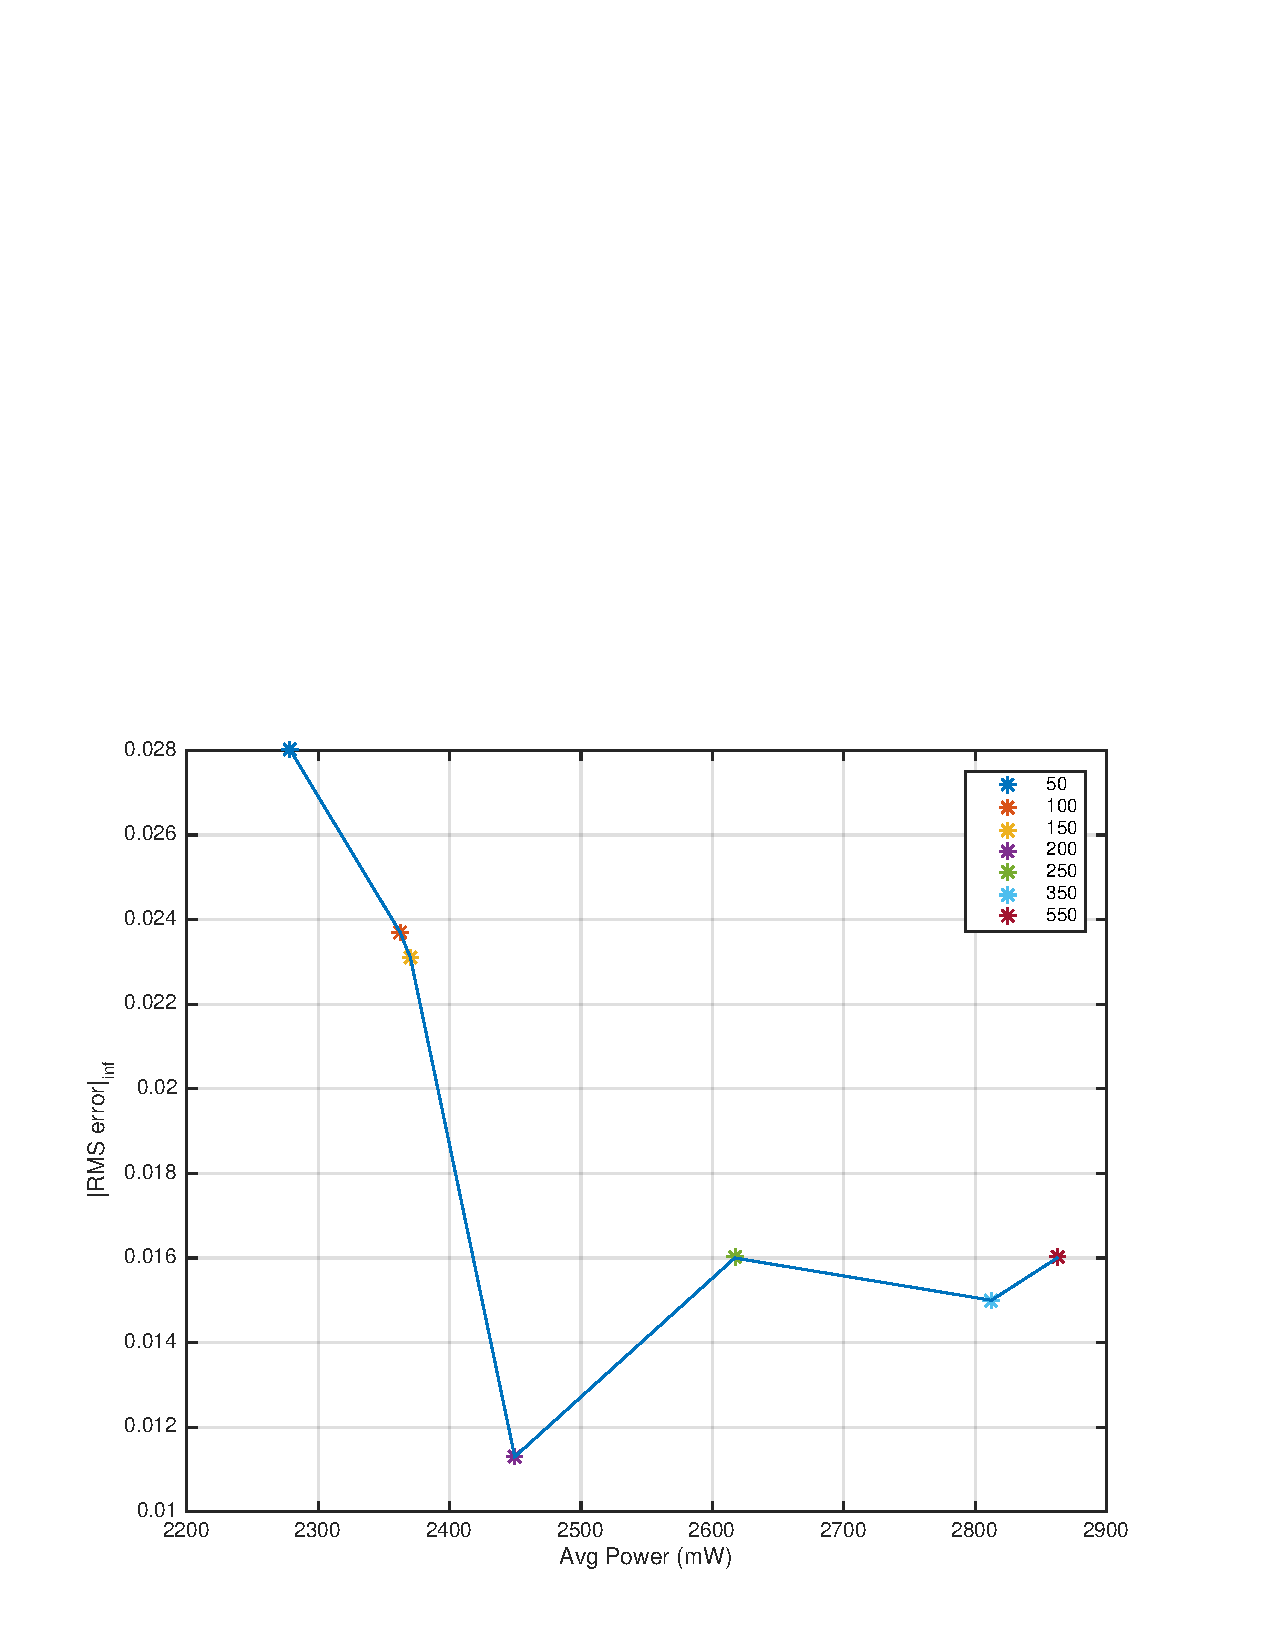
\includegraphics[width=0.9\columnwidth]{figures/errVsPower}
	\caption{Error vs power curve for the SVO algorithm running on the Odroid U3}
	\label{fig:svoErrVsPower}
\end{figure}

% subsection
%

\subsection{A contract time object recognition tool chain}

Our second example is a more complete perception tool chain shown in Fig.~\ref{fig:chain}.
\begin{figure}[t]
	\centering
	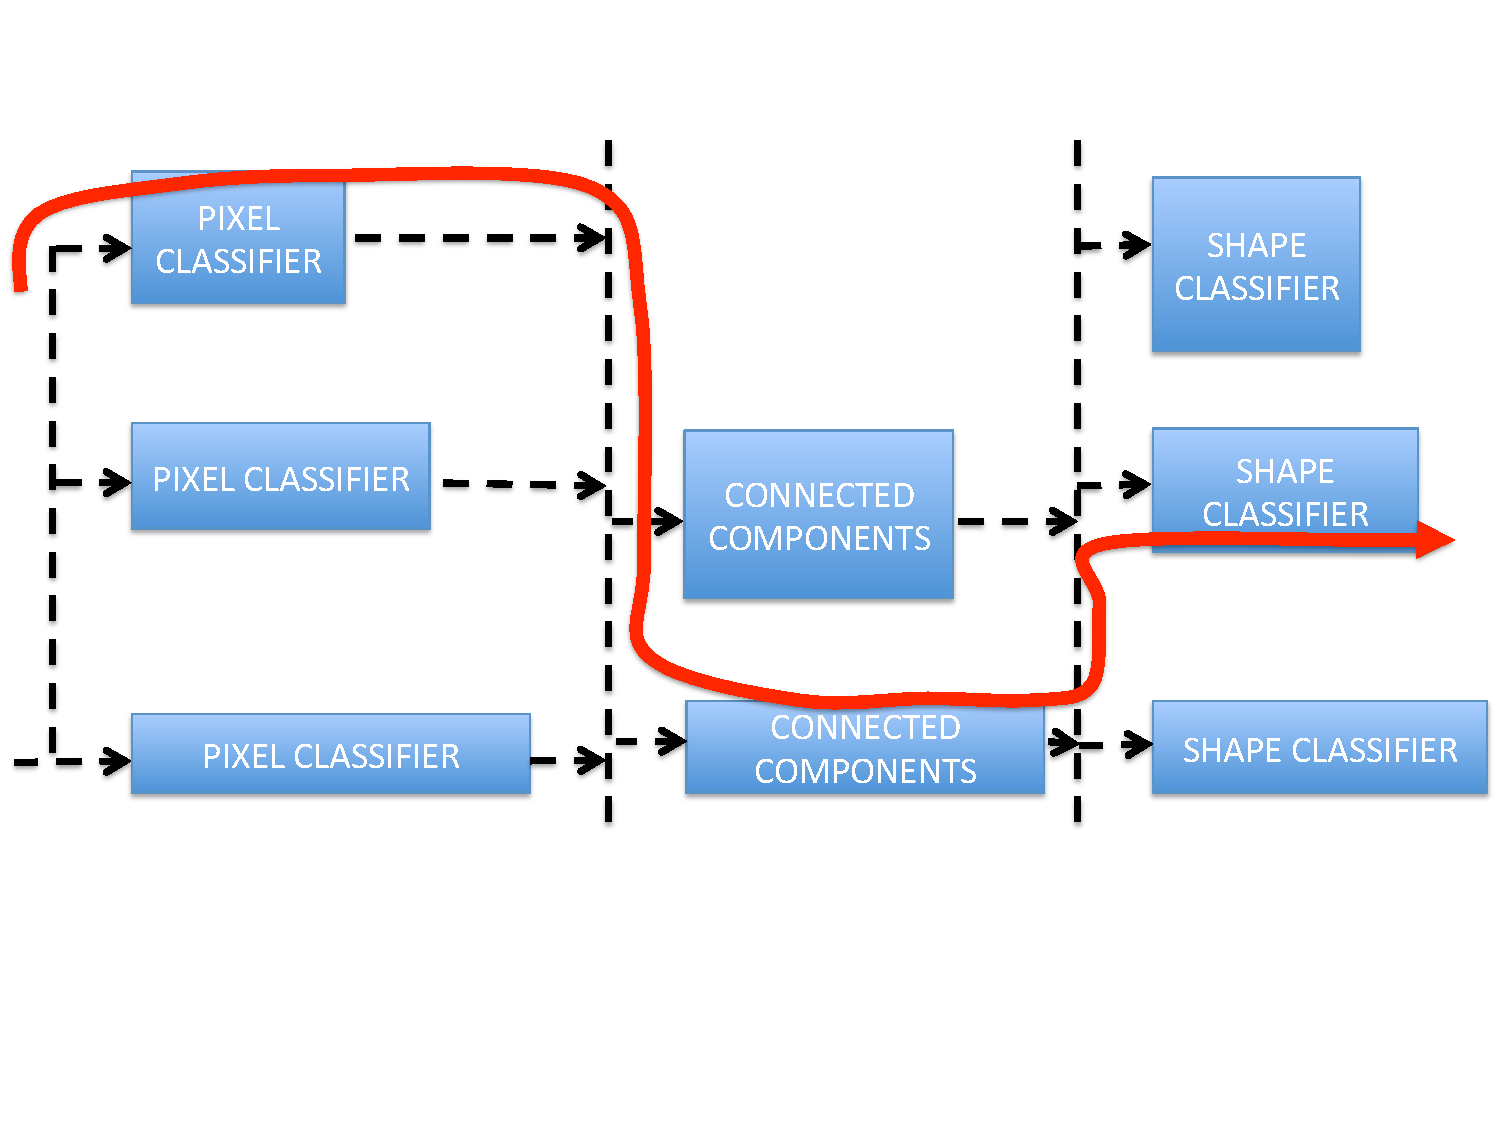
\includegraphics[width=0.7\linewidth]{figures/chain}
	\caption{Visual perception toolchain for object detection. The height of a block indicates output error, while width indicates runtime. The red path indicates one particular execution path which trades error for runtime at each stage.}
	\label{fig:chain}
\end{figure}
The tool chain takes in a video stream and tracks an Object Of Interest (OOI) across the frames.
The pixel classifier assigns to each pixel of the image (after potential pre-processing) the probability of its being a pixel of interest, i.e., of belonging to an OOI. 
A binary image is then obtained which assigns the value 1 to pixels of interest, and 0 to all others. 
A Connected Components (CC) algorithm is run on the binary image to segment its 1-valued pixels into disconnected objects.
A shape classifier is then run on each object to determine whether it is an object of interest or not.
The pixel and shape classifiers are machine learning algorithms that need to be trained on a training set before being used.
In our implementation of this chain, the specific algorithms and their knobs are as follows:
the pixel classifier is a Gaussian Mixture Model (GMMs), whose knob is the number of Gaussians in the mixture.
The connected components algorithm has a two-valued knob to choose between a 4-connected and 8-connected component implementation.
The shape classifier is also a GMM, but the knob for it is the number of shape features.
The number of Gaussian components for the shape classifier is fixed since we know in advance the number of objects in the training and test sets.
Thus the knob for the entire chain is $K$ = (\#Gaussians for pixel classifier, \#neighbors for CC, \#features for shape classifier), and has a total of $3 \times 2 \times 2 = 12$ values.
Note that for any given algorithm in the chain, the relation between knob value and quality of output is not necessarily monotonic. 
Like all machine learning algorithms, it will depend on the actual data set.
The same is a fortiori true of the quality of the output of the entire chain.

Fig.~\ref{fig:chainErrorDelay} shows the \emph{perception error}-delay curve for the object detection chain.
The perception error is the difference between the estimated centroid of the OOI and the true centroid of the OOI.
If the chain fails at finding the object in the frame, we assign that frame a constant error drawn from the errors found on other frames.
Each point on the curve was obtained by training the tool chain with the associated knob value, and then running the trained tool chain on the test set to obtain the $(\delta,\epsilon)$ values.
The plotted error value is the average error over all images in the test set.
The fact that the error \emph{increases} in some points despite increasing computation time can be explained by the remark made earlier: namely that the effect of a knob value is not necessarily monotonic on quality.
Moreover, the effect of a change to one algorithm of the chain might outweigh changes to other algorithms.
This makes profiling the end-to-end tool chain all the more important.
Thus, online, the controller can ignore the modes that show a degraded performance despite a higher energy cost.

This curve can then be turned into an estimate error-delay curve by incorporating it into an estimation algorithm.
\begin{figure}[t]
	\centering
	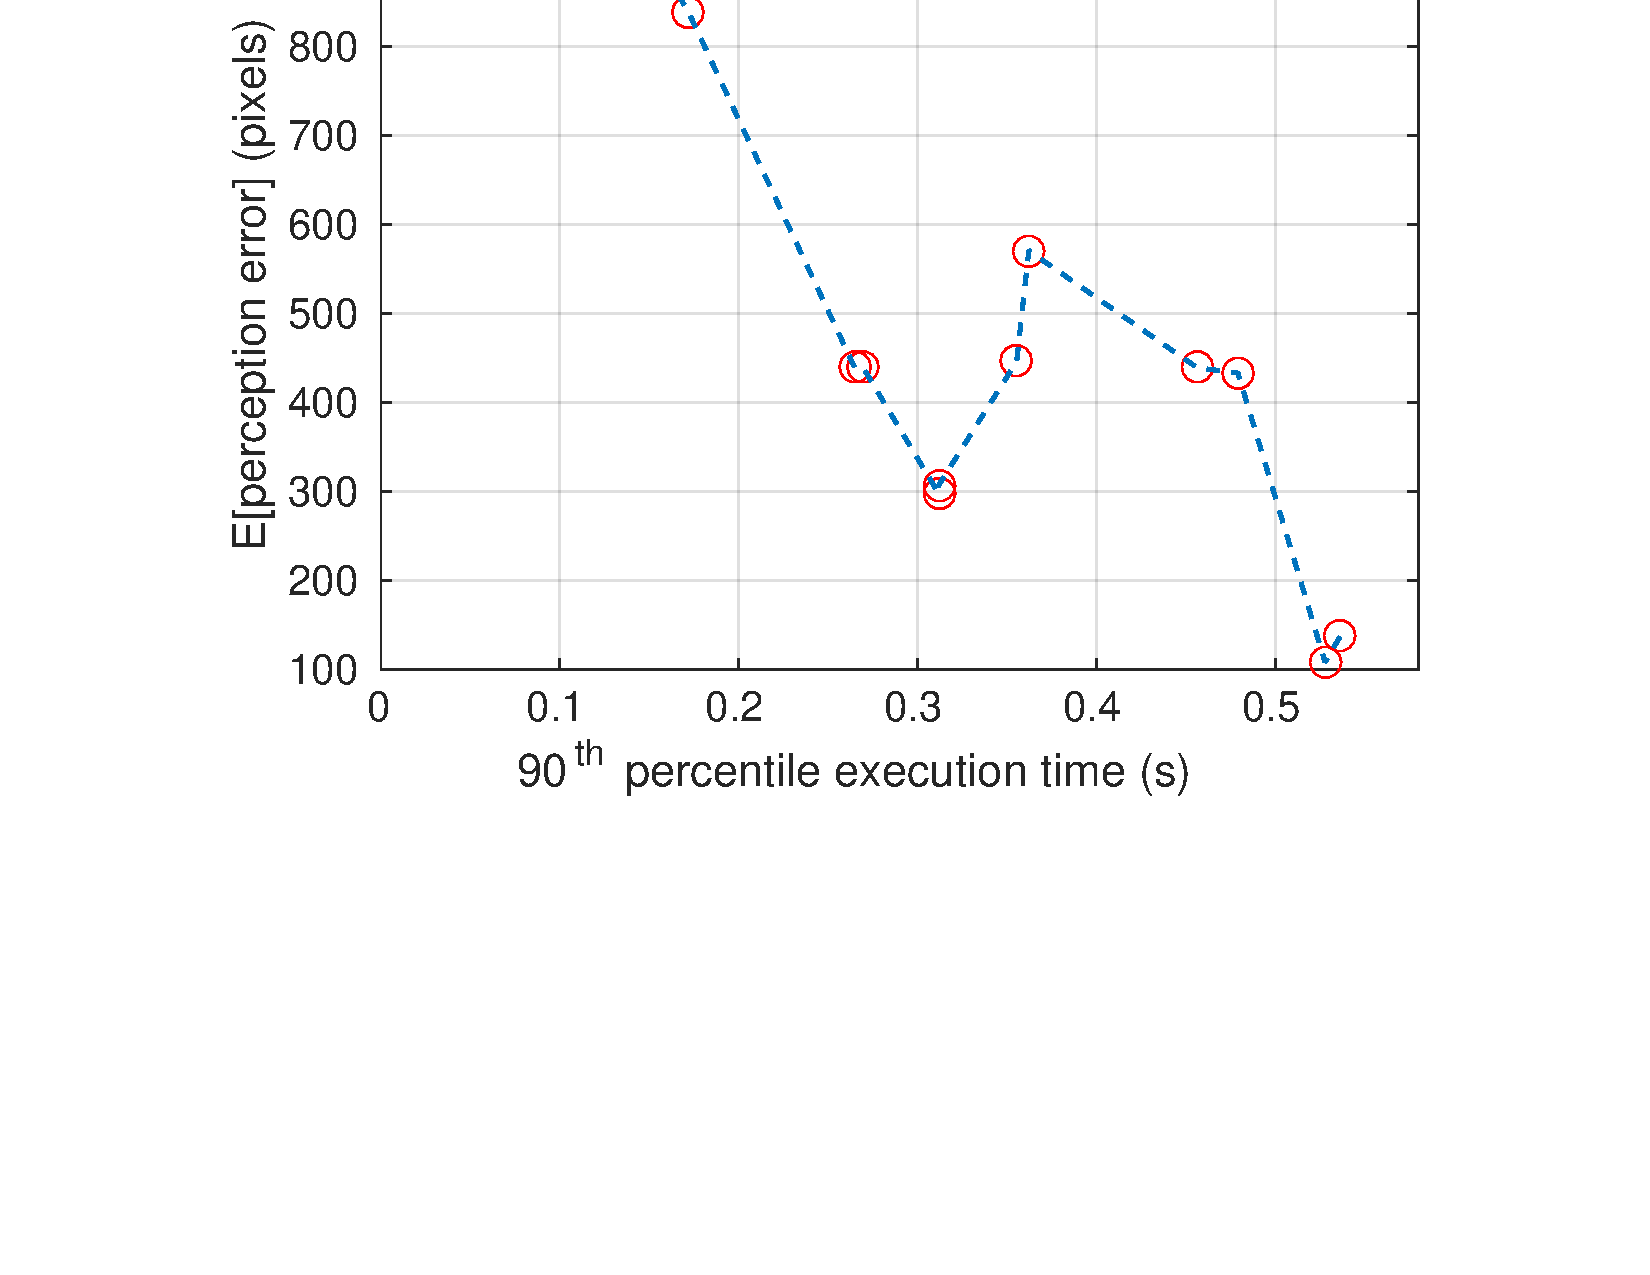
\includegraphics[width=0.7\linewidth]{figures/chainErrorDelay}
	\caption{Perception error vs Delay curve for the chain of Fig.~\ref{fig:chain}}
	\label{fig:chainErrorDelay}
\end{figure}
More generally, such curves can be obtained for a given state estimator by identifying the knobs that control the quality and runtime of the estimator, and profiling the estimator's code at the various values of the knobs.
In effect, this gives us several Estimator tasks, each with a different utility. 
I.e., each such task strikes a different balance between computation time and quality of estimate.
At time step $k$, the controller schedules the task with the best trade-off for step $k+1$, in the sense of optimizing the cost function in Eq.??


